\thispagestyle{empty}
\vphantom{}
\vfill{}
\newcommand\bordes{43}
\newcommand\tam{2.1cm}
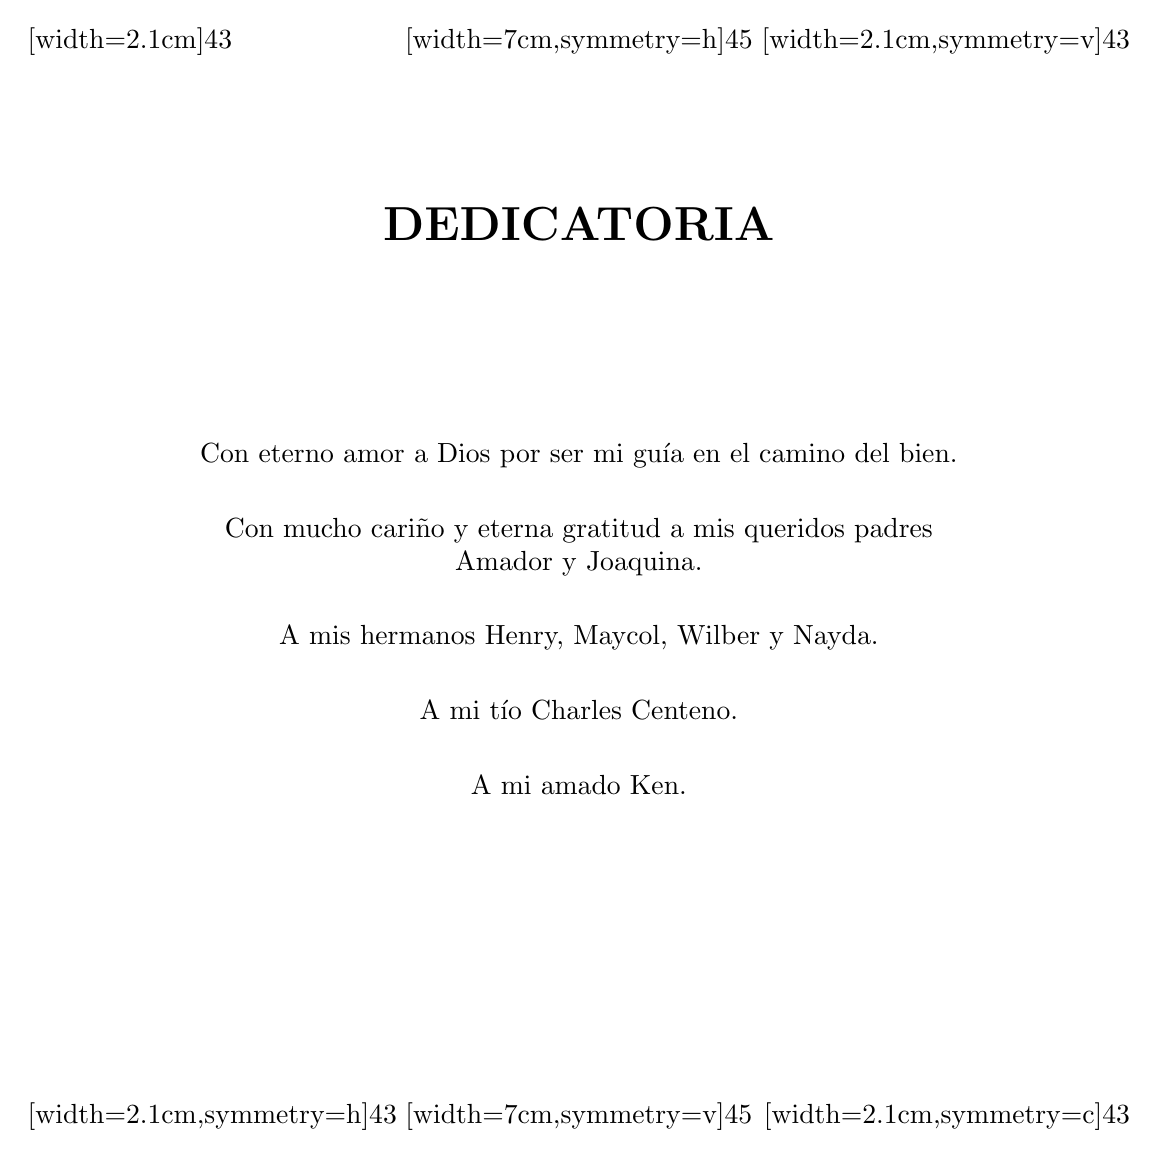
\begin{tikzpicture}[color=black,
	every node/.style={inner sep=0pt}]
	%\draw[help lines] (-6,-6) grid (6,6);
		\node[minimum size=14cm](vecbox){};

		\node[anchor=north west] at (vecbox.north west)
			{\pgfornament[width=\tam]{\bordes}};
		
		\node[anchor=north east] at (vecbox.north east)
			{\pgfornament[width=\tam,symmetry=v]{\bordes}};
		
		\node[anchor=south west] at (vecbox.south west)
			{\pgfornament[width=\tam,symmetry=h]{\bordes}};
		
		\node[anchor=south east] at (vecbox.south east){
			\pgfornament[width=\tam,symmetry=c]{\bordes}};
		
		%\node[anchor=north, rotate=-90] at (vecbox.east){
		%	\pgfornament[width=8cm,symmetry=h, ]{49} };
		
		\node[anchor=north] at (vecbox.north){
			\pgfornament[width=7cm,symmetry=h]{45}};
		
		\node[anchor=south] at (vecbox.south){
			\pgfornament[width=7cm,symmetry=v]{45}};
			
	%%%%%%%%%%%%%%%%%%%%% MODIFICAR TEXTO %%%%%%%%%%%%%%%%%%%%
	
		\node[minimum size=2cm,xshift=0cm, yshift=4.5cm](dedicatoria){\LARGE \textbf{DEDICATORIA}};
		
		\node[minimum size=8cm, align=center, line width=0pt, anchor=north] at (dedicatoria.south){
			Con eterno amor a Dios por ser mi gu\'ia en el camino del bien.\\[1.5em]
			Con mucho cari\~no y eterna gratitud a mis queridos padres \\ Amador y Joaquina.\\[1.5em]
			A mis hermanos Henry, Maycol, Wilber y Nayda.\\[1.5em]
			A mi t\'io Charles Centeno.\\[1.5em]
			A mi amado Ken.
		};
	
\end{tikzpicture}
\vfill{}
